\newpage
%\null
%\cleardoublepage



%************************************************************************************************
% Kap.3 Mathematische Modellbildung
%************************************************************************************************

\chapter{Mathematische Modellbildung}
\label{chap:modellbildung}

\section{Das System}
\label{chap:system}
Der vorliegenden Simulationsstudie wird in folgendes, in \ref{fig:aufbau_system} dargestellen Systems zugrunde gelegt.
\begin{figure}[ht]
	\centering
	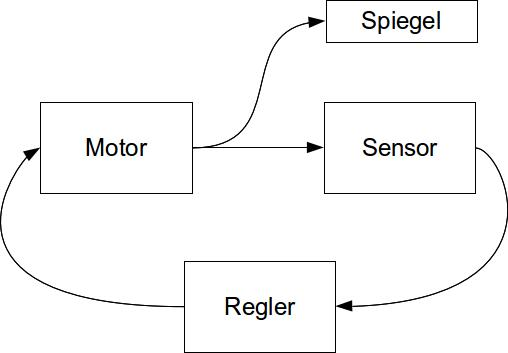
\includegraphics[width=0.6\textwidth]{System_Aufbau.jpg}
	\caption{Allgemeiner Aufbau des simulierten Systems}
	\label{fig:aufbau_system}
\end{figure}


\section{Der Motor}
\label{chap:motor}
In der Regel werden Laserablenkespiegel �ber einen Galvo gesteuert. Bei der Bearbeitung dieser Simulationsstudie ergaben sich Probleme, Informationen �ber die Ansteuerung
solcher Galvos zu bekommen. Insofern wird die Simulationsstudie auf der Ansteuerung eines Gleichstrommotors beruhen. Aber auch hierbei konnten jedoch keine Informationen 
�ber die Gleichstrommotorparameter KPHI und der Reibungskonstanten bei verschiedenen Herstellern gefunden werden. Um dennoch die Studie durchf�hren zu k�nnen, wird auf die
Motorvorgaben aus der Vorlesung Systemtechnik von Prof. Froriep zur�ck gegriffen.

Lineares Modell f�r die Berechnungen:

\begin{center}
\begin{equation}
\label{equ:lineares_motor_model}
\Delta \phi = 20{\textdegree} = 0,349 rad\\
\Delta t = 1 ms = 0,001 s\\
\omega = \frac {\Delta \phi}{\Delta t} = \frac {0,349 rad}{0,001 s} = 349 rad/s\\
\end{equation}
\end{center}
Es ergibt sich eine Druchschnittswinkelgeschwindigkeit von 349 rad/s, um einen Winkel von 20{\textdegree} in 1 ms zu �berfahren.
Dies w�rde aber eine Anfangs- und Endgeschwindigkeit voraussetzen. Da der Spiegel aber aus einer Ruhelage beschleunigt werden und wieder in einer Ruhelage enden soll, 
wird ein linearer Verlauf der Geschwindigkeit von $\omega = 0 rad/s$ und der doppelten Durchschnittsgeschwindigkeit $\omega = 698 rad/s$ bei der H�lfte der Strecke und bei 
der Endposition wieder $\omega = 0 rad/s$ der zu fahrenden Strecke angenommen. 
Daraus folgt eine Beschleunigung von:
\begin{center}
\begin{equation}
\label{equ:max_alpha_motor}
\Delta \omega = 698 rad/s\\
\Delta t = 0,5 ms = 0,0005 s\\
\alpha = \frac {\Delta \omega}{\Delta t} = \frac {698 rad/s}{0,0005 s} = 1,396 *10^6 rad/s^2\\
\end{equation}
\end{center}
Der Spiegel erf�hrt zu Beginn der Regelung eine Beschleunigung von $\alpha = 1,396 *10^6 rad/s^2$ um nach der H�lfte der Zeit, also nach 0,5 ms wieder mit dem gleichen
Betrag der Beschleunigung abgebremst zu werden.

Modell f�r den Spiegel:
Durchmesser: 12 mm --> Radius: R = 6 mm
H�he: h = 2 mm
Gewicht: m = 10g

Tr�gheitsmoment des Spiegels: 
\begin{center}
\begin{equation}
\label{equ:J_spiegel}
J = \frac {1}{4} * m * R^2 + \frac {1} {12} * m * h^2\\
J = \frac {1}{4} * 10*10^{-3} * (6*10^{-3})^2 + \frac {1} {12} * 10*10^{-3} * (2*10^{-3})^2\\
J = 93,3 * 10^{-9} kg m^2
\end{equation}
\end{center}

Aus den oben berechneten Daten ergibt sich ein Lastmoment von:
\begin{center}
\begin{equation}
\label{equ:M_last}
M_L = J * \alpha\\
M_L = 93,3 * 10^{-9} kg m^2 * 1,396 *10^6 rad/s^2 \\
M_L = 130,25 * 10^{-3}
\end{equation}
\end{center}

Theoretsiche Maximale Leistung eines Gleichstrommotors:
\begin{center}
\begin{equation}
\label{equ:max_leistung_motor}
P = M_L * \omega\\
P = 130,25 * 10^{-3} * 698 rad/s \\
P = 91 W
\end{equation}
\end{center}

\section{Der Sensor}
\label{chap:sensor}
Im Folgenden werden der Aufbau, das physikalische Modell, sowie verschiedene mathematische Modelle des Sensors vorgestellt und erl�utert.

\subsection{Das physikalische Modell des Sensors}
\label{chap:physik_modell_sensor}


\subsection{Das lineare Sensormodell}
\label{chap:linear_sensor}


\subsection{Das nicht lineare Sensormodell}
\label{chap:nonlinear_sensor}